%%%%%%%%%%%%%%%%%%%%%%%%%%%%%%%%%%%%%%%%
% Structured General Purpose Assignment
% LaTeX Template
%
% This template has been downloaded from:
% http://www.latextemplates.com
%
% Original author:
% Ted Pavlic (http://www.tedpavlic.com)
%
% Note:
% The \lipsum[#] commands throughout this template generate dummy text
% to fill the template out. These commands should all be removed when 
% writing assignment content.
%
%%%%%%%%%%%%%%%%%%%%%%%%%%%%%%%%%%%%%%%%%

%----------------------------------------------------------------------------------------
%       PACKAGES AND OTHER DOCUMENT CONFIGURATIONS
%----------------------------------------------------------------------------------------

\documentclass{article}

\usepackage{fancyhdr} % Required for custom headers
\usepackage{lastpage} % Required to determine the last page for the footer
\usepackage{extramarks} % Required for headers and footers
\usepackage{graphicx} % Required to insert images
\usepackage{lipsum} % Used for inserting dummy 'Lorem ipsum' text into the template
\usepackage[table]{xcolor}% http://ctan.org/pkg/xcolor

\usepackage{amsmath}

% Margins
\topmargin=-0.45in
\evensidemargin=0in
\oddsidemargin=0in
\textwidth=6.5in
\textheight=9.0in
\headsep=0.25in 

\linespread{1.1} % Line spacing

% Set up the header and footer
\pagestyle{fancy}
\lhead{\hmwkAuthorName} % Top left header
\chead{\hmwkClass\ : \hmwkTitle} % Top center header
\rhead{\firstxmark} % Top right header
\lfoot{\lastxmark} % Bottom left footer
\cfoot{} % Bottom center footer
\rfoot{Page\ \thepage\ of\ \pageref{LastPage}} % Bottom right footer
\renewcommand\headrulewidth{0.4pt} % Size of the header rule
\renewcommand\footrulewidth{0.4pt} % Size of the footer rule
\newcommand\numberthis{\addtocounter{equation}{1}\tag{\theequation}}
\setlength\parindent{0pt} % Removes all indentation from paragraphs

%----------------------------------------------------------------------------------------
%       DOCUMENT STRUCTURE COMMANDS
%       Skip this unless you know what you're doing
%----------------------------------------------------------------------------------------

% Header and footer for when a page split occurs within a problem environment
\newcommand{\enterProblemHeader}[1]{
\nobreak\extramarks{#1}{#1 continued on next page\ldots}\nobreak
\nobreak\extramarks{#1 (continued)}{#1 continued on next page\ldots}\nobreak
}

% Header and footer for when a page split occurs between problem environments
\newcommand{\exitProblemHeader}[1]{
\nobreak\extramarks{#1 (continued)}{#1 continued on next page\ldots}\nobreak
\nobreak\extramarks{#1}{}\nobreak
}

\setcounter{secnumdepth}{0} % Removes default section numbers
\newcounter{homeworkProblemCounter} % Creates a counter to keep track of the number of problems

\newcommand{\homeworkProblemName}{}
\newenvironment{homeworkProblem}[1][Problem \arabic{homeworkProblemCounter}]{ % Makes a new environment called homeworkProblem which takes 1 argument (custom name) but the default is "Problem #"
\stepcounter{homeworkProblemCounter} % Increase counter for number of problems
\renewcommand{\homeworkProblemName}{#1} % Assign \homeworkProblemName the name of the problem
\section{\homeworkProblemName} % Make a section in the document with the custom problem count
\enterProblemHeader{\homeworkProblemName} % Header and footer within the environment
}{
\exitProblemHeader{\homeworkProblemName} % Header and footer after the environment
}

\newcommand{\problemAnswer}[1]{ % Defines the problem answer command with the content as the only argument
\noindent\framebox[\columnwidth][c]{\begin{minipage}{0.98\columnwidth}#1\end{minipage}} % Makes the box around the problem answer and puts the content inside
}

\newcommand{\homeworkSectionName}{}
\newenvironment{homeworkSection}[1]{ % New environment for sections within homework problems, takes 1 argument - the name of the section
\renewcommand{\homeworkSectionName}{#1} % Assign \homeworkSectionName to the name of the section from the environment argument
\subsection{\homeworkSectionName} % Make a subsection with the custom name of the subsection
\enterProblemHeader{\homeworkProblemName\ [\homeworkSectionName]} % Header and footer within the environment
}{
\enterProblemHeader{\homeworkProblemName} % Header and footer after the environment
}
   
%----------------------------------------------------------------------------------------
%       NAME AND CLASS SECTION
%----------------------------------------------------------------------------------------

\newcommand{\hmwkTitle}{Midterm } % Assignment title
\newcommand{\hmwkDueDate}{Thursday,\ November\ 5,\ 2015} % Due date
\newcommand{\hmwkClass}{MATH-578B} % Course/class
\newcommand{\hmwkClassTime}{} % Class/lecture time
\newcommand{\hmwkAuthorName}{Saket Choudhary} % Your name
\newcommand{\hmwkAuthorID}{2170058637} % Teacher/lecturer
%----------------------------------------------------------------------------------------
%       TITLE PAGE
%----------------------------------------------------------------------------------------

\title{
\vspace{2in}
\textmd{\textbf{\hmwkClass:\ \hmwkTitle}}\\
\normalsize\vspace{0.1in}\small{Due\ on\ \hmwkDueDate}\\
\vspace{0.1in}\large{\textit{\hmwkClassTime}}
\vspace{3in}
}

\author{\textbf{\hmwkAuthorName} \\
        \textbf{\hmwkAuthorID}
        }
\date{} % Insert date here if you want it to appear below your name

%----------------------------------------------------------------------------------------

\begin{document}

\maketitle

%----------------------------------------------------------------------------------------
%       TABLE OF CONTENTS
%----------------------------------------------------------------------------------------

%\setcounter{tocdepth}{1} % Uncomment this line if you don't want subsections listed in the ToC

\newpage
\tableofcontents
\newpage



\begin{homeworkProblem}[Problem 1] % Roman numerals

\begin{homeworkSection}{\homeworkProblemName: ~(a)}
	\problemAnswer{
	$$
	P =	\begin{bmatrix}
			1-\alpha & \alpha\\
			\beta & 1-\beta
		\end{bmatrix}
	$$
		Let the stationary state be given by $\pi = (\pi_1,\pi_2)$, then:
		\begin{eqnarray*}
		\pi. P = \pi\\
		\pi_1 + \pi_2 =1
		\end{eqnarray*}
		
	Solving which gives:
	\begin{eqnarray*}
		(1-\alpha)\pi_1+\pi_2 = 1\\
		\pi_1 + \pi_2 = 1\\
		\implies (\pi_1,\pi_2) = (\frac{\beta}{\alpha+\beta}, \frac{\alpha}{\alpha+\beta}) 
	\end{eqnarray*}
	
	
	
		}
\end{homeworkSection}

\begin{homeworkSection}{\homeworkProblemName: ~(b)}
\problemAnswer{
	$\mathbf{w} = 101$ 
	\begin{eqnarray*}
	\beta_{w,w}(0) = 1\\
	\beta_{w,w}(1) = 0\\
	\beta_{w,w}(2) = 1
	\end{eqnarray*}
	
	\begin{eqnarray*}
	P_u(0) = 1\\
	P_u(1) = p_{w_2w_3} = p_{01} = \alpha\\
	P_U(2) = p_{w_1w_2}p_{w_2w_3} = p_{10}p_{01} = \beta\alpha\\
	\end{eqnarray*}
	
	Now,
	$$G_{w,w}(t) = \sum_{j=0}^2t^j\beta_{w,w}(j)P_{w,w}(j)$$
	
	Thus,
	\begin{align*}
	G_{w,w}(t) &= 1 \times 1 \times 1 + t \times 0 \times \alpha + t^2 \times 1 \times \beta \alpha\\ 
	&= 1+\alpha\beta t^2
	\end{align*}
	}
\end{homeworkSection}

\begin{homeworkSection}{\homeworkProblemName: ~(c)}
	\problemAnswer{
		$X_n$ : Number of occurrences(overlaps allowed)  in $A_1A_2A_3\dots A_n$
		Using Theorem $12.1$:
		$$
		\lim_{n \rightarrow \infty} \frac{1}{n} E(X_n) = \pi_w = \pi_1 \times p_{10} \times p_{01} = \frac{\beta}{\alpha+\beta} \times \beta \times \alpha = \frac{\alpha\beta^2}{\alpha+\beta}
		$$ 
		
		Thus $$	\lim_{n \rightarrow \infty} \frac{X_n}{n} = \frac{\alpha\beta^2}{\alpha+\beta}$$
		
		}
\end{homeworkSection}

\begin{homeworkSection}{\homeworkProblemName: ~(d)}

\problemAnswer{ % Answer
Spectral decomposition of $P$:

$$
det\begin{bmatrix}
\alpha-\lambda & 1-\alpha\\
1-\beta & \beta-\lambda
\end{bmatrix} = 0
$$

$$
\lambda^2 +(\alpha + \beta-2) \lambda + (1-\alpha -\beta) = 0
$$

Thus, $\lambda_1 = 1$ and $\lambda_2 = 1-\alpha-\beta$

Eigenvectors are given by:

$v_1^T = \big( x_1\ x_1 \big)\ \forall\ x_1 \in R$

and for $\lambda_2$ , $v_2 = \big( x_1\ \frac{-\beta x_1}{\alpha} \big)$

Now using Markov property: $P(X_n=1|X_0=0) = (P^n)_{01}$

Now, 

$P^n = VD^nV^{-1}$

where:
$$
V = \begin{bmatrix}
1 & 1\\
1 & \frac{-\beta}{\alpha}
\end{bmatrix}
$$

and 

$$
D = \begin{bmatrix}
1 & 0 \\
0 & (1-\alpha-\beta)
\end{bmatrix}
$$

$$
V^{-1} = \frac{-1}{\frac{\beta}{\alpha}+1}\begin{bmatrix}
-\frac{\beta}{\alpha} & -1 \\
-1 & 1
\end{bmatrix}
$$

Thus,

$$
P^n = \begin{bmatrix}
1 & 1\\
1 & \frac{-\beta}{\alpha}
\end{bmatrix} \times \begin{bmatrix}
1 & 0 \\
0 & (1-\alpha-\beta)^n
\end{bmatrix} \times \frac{-1}{\frac{\beta}{\alpha}+1}\begin{bmatrix}
-\frac{\beta}{\alpha} & -1 \\
-1 & 1
\end{bmatrix}
$$

$$
P^n = \frac{1}{\alpha+\beta} \begin{bmatrix}
\beta + \alpha(1-\alpha-\beta)^n & \alpha-\alpha(1-\alpha-\beta)^n\\
\beta - \beta(1-\alpha-\beta)^n & \alpha + \beta(1-\alpha-\beta)^n
\end{bmatrix}
$$


\underline{\textbf{ALITER}}

We consider the following identity: $P^{n+1}=PP^n$

then:

$$
\begin{bmatrix}
p_{00}^{n+1} & p_{01}^{n+1}\\
p_{10}^{n+1} & p_{11}^{n+1}\\
\end{bmatrix} = \begin{bmatrix} 
p_{00}^n & p_{01}^n\\
p_{10}^n & p_{11}^n
\end{bmatrix} \times \begin{bmatrix}
1-\alpha & \alpha\\
\beta & 1-\beta
\end{bmatrix}
$$

$\implies$


\begin{align*}
p_{11}^{n+1} &= p_{10}^n(\alpha) + p_{11}^n(1-\beta)\\
&= (1-p_{11}^n)(\alpha) +(p_{11}^n)(1-\beta)\\
&= \alpha + (1-\alpha-\beta)p_{11}^n   \tag{1d.1}
\end{align*}

}
\clearpage
\problemAnswer{

On similar lines:

\begin{align*}
p_{00}^{n+1} &= (1-\alpha-\beta)p_{00}^n + \beta   \tag{1d.2}
\end{align*}

In order to solve equations of type $1d.1$ and $1d.2$ we take the following strategy:

By substituting $p_{00}^{n+1} = p_{00}^n$ (and thus obtaining the stationary solution at $\frac{\beta}{\alpha+\beta}$), $1d.2$ can be reduced to the following form:

\begin{align*}
p_{00}^{n+1} &= \frac{\beta}{\alpha+\beta}= (1-\alpha-\beta)(p_{00}^n -\frac{\beta}{\alpha+\beta})  \label{1d.3}
\end{align*}




Let's call $y^(n) =  p_{00}^n -\frac{\beta}{\alpha+\beta}$


Then $1d.3$ is similar to:

\begin{eqnarray*}
y^{(n+1)} = (1-\alpha-\beta)y^(n) \\
y^{(n+1)} = (1-\alpha-\beta)^ny^(0)
\end{eqnarray*}

$y^(0) = p_{00}^{(0)} - \frac{\beta}{\alpha+\beta}$

Assume $p_{00}^{(0)}=1$ $\implies$ $y^{(0)} = \frac{\alpha}{\alpha+\beta }$

Which gives:

$$
p_{00}^n = (1-\alpha-\beta)^n \frac{\alpha}{\alpha+\beta} + \frac{\beta}{\alpha+\beta} \text{if $\alpha+\beta > 0$}
$$

Similarly,

$$
p_{11}^n = (1-\alpha-\beta)^n \frac{\beta}{\alpha+\beta} + \frac{\alpha}{\alpha+\beta} \text{if $\alpha+\beta > 0$}
$$

\textbf{NOTE:} If $\alpha+\beta = 0$, we get:
$$
P^n = \begin{bmatrix}
1 & 0\\
0 & 1
\end{bmatrix}
$$

}

\end{homeworkSection}

\begin{homeworkSection}{\homeworkProblemName: ~(e)}
\problemAnswer{
	$\pi_w =\pi_i p_{10}p_{01} = \frac{\alpha}{\alpha+\beta} \times \beta \alpha  =  \frac{\alpha^2\beta}{\alpha+\beta}$
	  
	\begin{align*}
	\lim_{n \rightarrow \infty} \frac{Var(X_n)}{n} &= 2\pi_w \big((\beta_{w,w}(0)P_w(0) -\pi_w ) + (\beta_{w,w}(1)P_w(1) - \pi_w ) + (\beta_{w,w}(2)P_w(2) - \pi_w )	\big)\\
	 &+ 2\pi_w P_w(2)\sum_{j=0}^\infty \{p^{j+1}_{11} - \pi_1 \} + \pi_w^2-\pi_w \\
	&= 2\frac{\alpha^2\beta}{\alpha+\beta} (1+\alpha\beta - 3\frac{\alpha^2\beta}{\alpha+\beta} )  + 2\frac{\alpha^2\beta}{\alpha+\beta}   \sum_{j=0}^\infty \{ \frac{\beta}{\alpha+\beta}(1-\alpha-\beta)^j  \} - \frac{\alpha^2\beta}{\alpha+\beta} + (\frac{\alpha^2\beta}{\alpha+\beta})^2\\
	%&=\frac{\alpha^2\beta}{\alpha+\beta} \big(2(1-2\alpha\beta) + 2 %(\beta+\frac{\alpha}{\alpha+\beta}) + \alpha\beta)
	&=\frac{\alpha^2\beta}{\alpha+\beta}(\frac{(2\alpha+2\beta -4\alpha^2\beta + 2\alpha\beta^2 +2\alpha\beta+2\beta^2+\alpha^2\beta-\alpha-\beta)}{\alpha+\beta} )\\
	&= \frac{\alpha^2\beta(\alpha+\beta-3\alpha^2\beta+2\alpha\beta^2+2\alpha\beta+2\beta^2)}{(\alpha+\beta)^2} 
	\end{align*}
		
}
\end{homeworkSection}



\begin{homeworkSection}{\homeworkProblemName: ~(f)}
	\problemAnswer{
		$Y_n$: Number of occurrences of word $w$ in all words, thus,
		$Y_n \approx c X_n$
		
		\textbf{NOTE:} I assume the problem should be to estimate $\lim_{n \rightarrow \infty} \frac{Y_n}{n}$ and $\lim_{n \rightarrow \infty } \frac{Var(Y_n)}{n}$ In the problem it mentions $X_n$ instead of $Y_n$
		
		Thus,
		\begin{align*}
			\lim_{n \rightarrow \infty} \frac{Y_n}{n} &= c \times \lim_{n \rightarrow} \frac{X_n}{n}\\  
			&= c\frac{\alpha^2\beta}{\alpha+\beta} \\
			\lim_{n \rightarrow \infty } \frac{Var(Y_n)}{n} &= c^2 \times \lim_{n \rightarrow \infty } \frac{Var(X_n)}{n}\\ 
			&= c^2 \times \big( \frac{\alpha^2\beta(\alpha+\beta-3\alpha^2\beta+2\alpha\beta^2+2\alpha\beta+2\beta^2)}{(\alpha+\beta)^2}  \big)
		\end{align*} 
		
		Please see Appendix 1 for code and report.
		
		}
\end{homeworkSection}
\end{homeworkProblem}

\begin{homeworkProblem}[Problem 2]
\begin{homeworkSection}{\homeworkProblemName: ~(a)}
	\problemAnswer{
		Expected number of squares of side length $t$ such that all $X_v$ are 1 in the square: We simply choose a position on the positive lattice $x$ axis and then construct a square around it $[(x_0,y_0) (x_0+t,y_0+t)]$ so we have $n-t+1$ choices for $x_0$ and $n-t+1$ choices for $y_0$, the constraint being that all points inside are all $1$, there are approximately $t^2$ integer points inside 
		
		$$
		E(\# \text{number of squares of side length $t$ such that all $X_v$ are 1 inside}) = (n-t) \times (n-t) p^{t^2} = (n-t+1)^2 p^{t^2}
		$$
		
		More formally, we define the indicator $C_{i,j} = I(X_{i+p,j+q}=1)$ $\forall 0 \leq p,q \leq t-1$
		
		and hence $E(Y_t) = E(\sum_{i=0}^{n-t+1}\sum_{j=0}^{n-t+1}C_{i,j}(t)) = (n-t+1)^2p^{t^2}$ 
		
	}
\end{homeworkSection}

	
	\begin{homeworkSection}{\homeworkProblemName: ~(b)}
		\problemAnswer{
			
			Just like the largest run problem, this problem should satisfy 
			\begin{align*}
			(n-t)^2  \times p^{T^2} &= 1\\
			\implies \lim_{n \rightarrow \infty }(n^2) p^{T_n^2} = \frac{1}{n^2}\\
			\lim_{n \rightarrow \infty } \log_{1/p}p^{T^2} &= \log_{1/p}(\frac{1}{n^2})\\
			\lim_{n \rightarrow \infty }T_n^2 &= 2 \log_{1/p}(n)\\
			\lim_{n \rightarrow \infty } \frac{T_n}{\sqrt{2\log_{1/p}(n)}} &=1
			\end{align*}
			
			Thus, $$a(n) = \sqrt{2\log_{1/p}(n)}$$

			
			}
	\end{homeworkSection}
	
\begin{homeworkSection}{\homeworkProblemName: ~(c)}
\problemAnswer{
	For declumping: 
	\begin{align*}
	W_(1,1) &=1\\
	W_{i,j} &=  (1-\prod_{p=0} I(X_{i+p,j-1}=1)I(X_{i-1,j+p}=1)) \times \prod_{p=0}^{t-1} \prod_{q=0}^{t-1}I(X_{i+p,j+q}=1) \\
	W_(i,j) &= C_{i,j}(t-1) - C_{i,j}(t)
	\end{align*}
	
	
	The set $I$ is given by: $I = \{(i,j): 0 \leq i,j \leq n-t+1 \}$
	The dependence set for $\nu=(i,j)$ is given by $J_\nu = \{(i',j') \in I: |i-i'| \leq t \text{and } |j-j'| \leq t \}$

Now, 
\begin{align*}
b_1 &= \sum_{i \in I} \sum_{j \in J_i} E(X_i)E(X_j)\\
&= (n-t+1)^2 \times (2t+1)^2  \times(p^{(t-1)^2}-p^{(t)^2	})
\end{align*}
	
And,

\begin{align*}
b_2 &= \sum_{i \in I}\sum_{ i\neq j \in J_i}E(X_iX_j)\\
&= 0
\end{align*}
	
	In order to choose a $t(n)$ such that $W$ is approximately poisson with $\lambda = (n-t+1)^2(p^{(t-1)^2}-p^{t^2})$, choose $t_n = \sqrt{(2\log_{1/p}(n))}$ so that $b1 \rightarrow 0$ (because $b1 = \frac{(2t+1)^2\lambda^2}{(n-t+1)^2} \rightarrow \frac{\log(n)}{n^2} \rightarrow 0 $)  and hence by Thorem $11.22$, we have $W$ to be  a poisson(since $b_1=b_2=0$)
	}
\end{homeworkSection}
\end{homeworkProblem}

\begin{homeworkProblem}[Problem 3]
	\begin{homeworkSection}{\homeworkProblemName: ~(a)}
		\problemAnswer{
			\begin{align*}
			P(A_i=B_i) &= \sum_{a \in S} \eta_a \gamma_a 
 			\end{align*}
 			}
	\end{homeworkSection}

	\begin{homeworkSection}{\homeworkProblemName: ~(b)}
		\problemAnswer{
			If $X_i$ is the the number of matches between two consecutive matches, it follows a \textbf{negative binomial} distribution(Intuition: Number of successes are $X_i$ before the first failure occurs(and then everything resets!))
			
			$X_i \sim NB(1,p) $ which is basically a geometric distribution.
			And hence $P(X_i=k) = (1-p)^kp$
			
		}
	\end{homeworkSection}
	
		
	\begin{homeworkSection}{\homeworkProblemName: ~(c)}
		\problemAnswer{
			From Theorem 11.18, if $X_1,X_2 \dots X_n$ are i.i.d
			then
			\begin{align*}
		\lim_{n \rightarrow \infty} P(Y_n < a_n+b_ny) = e^{-u(y)} \tag{3c.1}
			\end{align*}
				
			where,
			\begin{align*}
			\lim_{n \rightarrow \infty} n\{1-F(a_n+b_ny)\} = u(y)   \tag{3c.2}
			\end{align*}

			
			
			We have: $F(X) = P(X \leq x) = 1-p^x$
			
			Now ,
			
			\begin{align*}
			\lim_{n \rightarrow \infty} P\{b_n(Y_n-a_n) \leq z \} = \exp(-\exp(z))\\
			\lim_{n \rightarrow \infty} P\{(Y_n \leq \frac{1}{b_n}z + a_n \} = \exp(-\exp(z)) \tag{3c.3} 
			\end{align*}
			
			Thus, comparing coefficients in $(3c.1),(3c.2),(3c.3)$, we have:
			\begin{align*}
			\lim_{n \rightarrow \infty} n(1-F(a_n+\frac{1}{b_n}z))  &= \exp(-z)\\
			\lim_{n \rightarrow \infty} n(1-(1-p^{a_n+\frac{1}{b_n}z}))  &= \exp(-z)\\
			\lim_{n \rightarrow \infty}  np^{a_n + \frac{1}{b_n}z} & = \exp(-z)
			\lim_{n \rightarrow \infty}  (np^{a_n})  (p^{\frac{1}{b_n}} e)^z & = 1
			\end{align*}
			
			Satisfying which requires:
			\begin{align*}
			np^{a_n} &= 1\\
			1/p^{a_n} &= n\\
			\implies a_n &= \log_{1/p}(n)	
			\end{align*}
			
			And,
			\begin{align*}
			(p^{\frac{1}{b_n}} e)^z & = 1\\
			z (\log(p^{\frac{1}{b_n}}) + 1) &= 0\\
			\implies b_n &= \log(1/p)
			\end{align*}
			
			Thus, \begin{align*}
			a_n &= \log_{1/p}(n)\\
			b_n &= \log(1/p)
			\end{align*}
		}
	\end{homeworkSection}
	
	\begin{homeworkSection}{\homeworkProblemName: ~(d)}
		\problemAnswer{
			$E(M_n) = n(1-p) = nq$
			Now, with similar calculations as in the last part it is possible to show that this follows an extreme value distribution:
			$$
			P\{\log(1/p) (Y_n-\log_{1/p}(nq))  < z\} \rightarrow \exp(-\exp(-z))
			$$
			
		}
	\end{homeworkSection}
	
	\begin{homeworkSection}{\homeworkProblemName: ~(e)}
		\problemAnswer{
			\textbf{Part(i)}
			
			\begin{align*}
			E(s(A,B)) &= \eta_0\gamma_0\times s(0,0) + \eta_1\gamma_0\times s(1,0) + \eta_0\gamma_1\times s(0,1) + \eta_1\gamma_1\times s(1,1)\\
			&= \frac{1}{3} + \frac{1}{6} -2\frac{1}{6} -2\frac{1}{3}\\
			&= -\frac{1}{2}
			& < 0
			\end{align*}
		
		\textbf{Part (ii)}
		
		To calculate such a $\lambda$ such that $\lambda(R_n-\ln(K_n)) $ has extreme value distribution, we find roots of $E(e^{xS(A,B)})=1$
		
		$p = \sum_a \eta_a \gamma_a = \frac{1}{2}$
		
		So, $pe^\lambda + (1-p)e^{-2\lambda} = 1$ $\implies$ $e^\lambda + e^{-2\lambda} = 2$
		
	 thus, $t^2+t-2=0$ $t= \frac{-1\pm \sqrt{5}}{2}$ 
	 
	 And since $\lambda > 0$ $\implies $ $\lambda = \exp(\frac{1+\sqrt{5}}{2})$
	 
	 
	 \textbf{Part (iii)}
	 
	 In aligned part: $p_{ab} = \eta_a \gamma_b e^{\lambda s(a,b)}$
	 
	 \begin{align*}
	 p_{00} &= \frac{1}{3} \frac{1+\sqrt{5}}{2}\\
	 p_{01} &= \frac{1}{3} \big(\frac{1+\sqrt{5}}{2} \big)^{-2}\\
	 p_{10} &= \frac{1}{6} \big(\frac{1+\sqrt{5}}{2} \big)^{-2}\\
	 p_{11} &= \frac{1}{6} \big(\frac{1+\sqrt{5}}{2} \big)
	 \end{align*}	
		
		}
		
	\end{homeworkSection}

\end{homeworkProblem}



\begin{homeworkProblem}[Problem 4]
	\begin{homeworkSection}{\homeworkProblemName: ~(a)}
		\problemAnswer{
			$$
			P(n\text{ individuals with allele A}) = {N\choose {n}} f_A^n(1-f_A)^{N-n}
			$$
		}
	\end{homeworkSection}
	
	\begin{homeworkSection}{\homeworkProblemName: ~(b)}
		\problemAnswer{
			Coverage is $\lambda$, thus the probability that this particular locus does NOT
			get sequenced = $\exp(-c)$
		
		%Since there are $n$ individuals with allele 'A' and $N-n$ individuals with allele 'a',
		%the only way to NOT see any read with allele 'A' and 'a' is that the locus does not get sequenced. We ignore any sequencing errors. Hence the only way no reads coming from the $n$ individuals do not have 'A' is that ALL of them do not sequence the specific locus and likewise for allele 'a' in $N-n$ individuals.
		
		\begin{align*}
		P(\text{At least one read with allele 'A' AND 'a'} ) &= 1 -P(\text{ Zero reads with allele 'A' OR 'a'}) \\
		&= 1-P(\text{Zero reads with 'a'})\\
		&- P(\text{Zero reads with allele 'A'})\\
		&+P(\text{Zero reads with allele 'A' and 'a'})\\
		&= 1 - (\exp(-\lambda))^n - (\exp(-\lambda))^{N-n} + (\exp(-\lambda))^n\\
		&= 1 - e^{-n\lambda} - e^{-\lambda(N-n)} + e^{-\lambda N}
		\end{align*}
		
		
		}
		
	\end{homeworkSection}
	
	
	\begin{homeworkSection}{\homeworkProblemName: ~(c)}
		\problemAnswer{
		For the locus to be declared polymorphic, there should be \emph{at least} one read with 'A' and \emph{at least} one read with allele 'a'. 
		
		\begin{align*}
		P(\text{locus is polymorhic}) &= 1 - P(\text{locus is not polymorphic})\\
		&= 1 - P(\text{ Zero reads with allele 'A' AND 'a'})\\
		&= 1 - e^{-n\lambda} - e^{-\lambda(N-n)} + e^{-\lambda N}
		\end{align*}
		
		}
	\end{homeworkSection}
	
\end{homeworkProblem}


\begin{homeworkProblem}[Problem 5]
	\begin{homeworkSection}{\homeworkProblemName: ~(a)}
		\problemAnswer{
			\begin{align*}
			L(n_{ii',jj'} | p_{00}p_{01}p_{10}p_{11}) & = \prod_{ii',jj'} \big(\alpha_{ii'jj'} p_{ij}p_{ij'}\big)^{n_{ii'jj'}} \\
			\alpha_{ii'jj'} &= \begin{cases}
			1 & (i=i';j=j')\\
			2 & (i=i'; j \neq j'\ OR\ i\neq i'; j=j' )\\
			4 & (i \neq i'; j \neq j')
			\end{cases}
			\end{align*}
			
			\centering{and $i,i',j,j' \in \{0,1\}$}
			
		
		}
	\end{homeworkSection}
	
	\begin{homeworkSection}{\homeworkProblemName: ~(b)}
		\problemAnswer{
			Missing Data?
			
			Let's look at the haplotypes:
			\begin{center}

			\begin{tabular}{|c|c|c|c|}
				\hline  & 00 &  01 & 11 \\ 
				\hline 00 & (00,00) &  (00,01)  & (01,01)  \\ 
				\hline 01 & (00,10) &  \cellcolor{yellow} (00,11);(01,10) & (00,10) \\ 
				\hline 11 & (10,10) &  (10,11)  & (11,11)  \\ 
				\hline 
			\end{tabular} 
			\end{center}

			Ambiguity in haplotypes occur whenever any of loci 'A,B' is heterozygous or both are heterozygous.
			
			$n_{10,10}$ in this case gives rise to twp haplotype pairs: $(11,00);(10,01)$ and %hence the missing data is $n_{(11/00)}$; $n_{(10/01)}$ since 
			We cannot directly determine the exact count from the genotype information. 
			In otherwords the haplotype counts $n_{(11/00)}$ and $n_{(10/01)}$ are  the missing data.
			
			Thus, missing data: $n_{00/11}$ and $n_{01/01}$.\\
			
			We assume there $N$ individuals and hence there are $2N$ haplotypes.\\
			
			\textbf{Observed data: }$Y=(n_{0000},n_{1100},n_{1111},n_{0001},n_{1101},n_{0111}, n_{0101})$\\
			
			\textbf{Missing Data}: %$n_{00};n_{01};n_{10}, n_{11}$ 
			$n_{00/11}$ and $n_{01/10}$ \\
			
			We construct complete data as the haplotype counts:\\
			\textbf{Complete Data:} $n_{00}, n_{01}, n_{10}, n_{11}$\\
			
			Parameters: $\theta= (p_{00},p_{01},p_{10},p_{11})$\\
			
			and hence the Complete data likelihood is given by:\\
			$$
			g(n_{00}, n_{01}, n_{10}, n_{11} | \theta ) = \frac{2N}{n_{00}!n_{01}!n_{10}!n_{11}!} p_{00}^{n_{00}}p_{01}^{n_{01}}p_{10}^{n_{10}}p_{11}^{n_{11}}
			$$
			
		}
	\end{homeworkSection}
	
	
	\begin{homeworkSection}{\homeworkProblemName: ~(c)}
		\problemAnswer{
			In the $E$ step. we perform ($m^{th}$ step):
			\begin{eqnarray*}
				\hat{n_{00}} = E[n_{00} | Y, \theta_m]\\
				\hat{n_{01}} = E[n_{01} | Y, \theta_m]\\
				\hat{n_{10}} = E[n_{10} | Y, \theta_m]\\
				\hat{n_{11}} = E[n_{11} | Y, \theta_m]\\
			\end{eqnarray*}
			
			
			where $\theta_m=(p_{00}^{(m)}, p_{01}^{(m)}, p_{10}^{(m)}, p_{11}^{(m)} )$
			
			Just consider $n_{00}$ for now.
			
			
			\begin{align*}
			n_{00} &= E[n_{00} | Y, \theta_m]\\
			&= 2n_{0000} +  n_{0010} + n_{0100} + E[n_{00/11}|Y,\theta_m]
			\end{align*}
			where the last term comes because the $00$ haplotype can also come from the ambiguos we highlighted in the table above $(11,00);(10,01)$
			
			Now, we need to consider:
			
			
			\begin{align*}
			E[n_{00/11}|Y,\theta_m] &= n_{0101} P({00/11}|{01/10},{00/11}) \\
			&= n_{0101} \times ( \frac{2p_{00}p_{11}}{2p_{00}p_{11}+2p_{01} p_{10}})
			\end{align*}
			
			Where the latter term comes out from the conditional probability of observing $01/10$ haploltype given it is coming from  a heterozygous subpopulation at both A,B
			
			Thus, the $E$ step gives us:
			
			\begin{align*}
			\hat{n_{00}} &= 2n_{0000} +  n_{0010} + n_{0100} + n_{0101} \frac{p_{00}p_{11}}{p_{00}p_{11}+p_{01} p{10}}\\
			\hat{n_{01}} &= 2n_{0011} + n_{0001} + n_{0100} + n_{0101}  \frac{p_{01}p_{10}}{p_{00}p_{11}+p_{01} p{10}}\\
			\hat{n_{10}} &= 2n_{1100} + n_{1000} + n_{1101} +  n_{0101}\frac{p_{10}p_{01}}{p_{00}p_{11}+p_{01} p{10}}\\
			\hat{n_{11}} &= 2n_{1111} + n_{1010} + n_{1110} +  n_{0101}\frac{p_{11}p_{00}}{p_{00}p_{11}+p_{01} p{10}}
			\end{align*}
			

			
		}
	\end{homeworkSection}
	
	\begin{homeworkSection}{\homeworkProblemName: ~(d)}
		\problemAnswer{
			$$
			g(n_{00}, n_{01}, n_{10}, n_{11} | \theta ) = \frac{2N}{n_{00}!n_{01}!n_{10}!n_{11}!} p_{00}^{n_{00}}p_{01}^{n_{01}}p_{10}^{n_{10}}p_{11}^{n_{11}}
			$$
			At the $M$ step, we maximise the likelihood function $(g)$ with respect to $\theta_m$, since it is a multinomial, and we know the the MLE for a multinomial is simply given by the ratio of $p_x = \frac{n_x}{N}$
			
			we get:
			\begin{eqnarray*}
			p_{00} = \frac{\hat{n_{00}}}{2N}\\
			p_{01} = \frac{\hat{n_{01}}}{2N}\\
			p_{10} = \frac{\hat{n_{10}}}{2N}\\
			p_{11} = \frac{\hat{n_{11}}}{2N}\\
			\end{eqnarray*}
			
		}
	\end{homeworkSection}
	\newpage
	\begin{homeworkSection}{\homeworkProblemName: ~(e)}
		\problemAnswer{
			%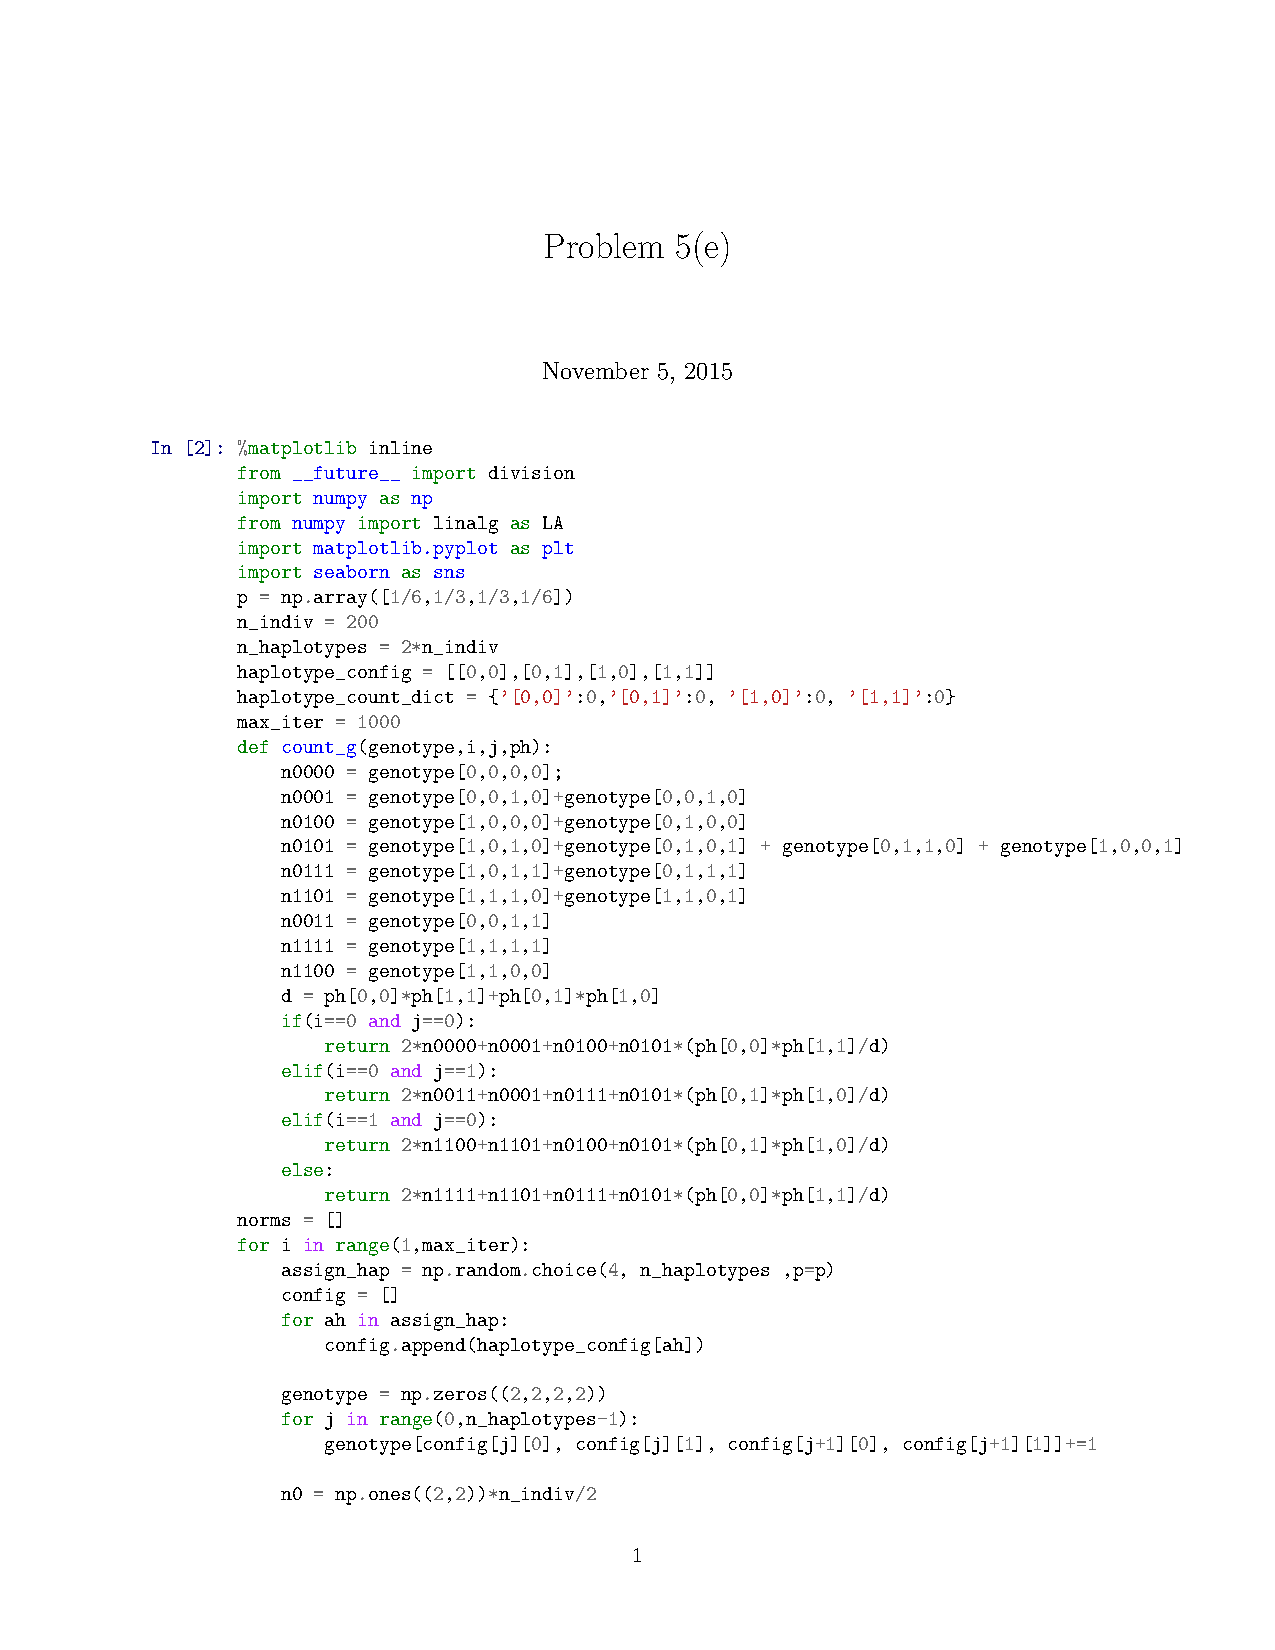
\includegraphics{Problem5/Problem5(e)}
			See Appendix 2.
		}
	\end{homeworkSection}
	
	\begin{homeworkSection}{\homeworkProblemName: ~(f)}
		\problemAnswer{
			
			Challenge: If there are $L$ loci, there are $2^L$ haplotypes and hence the EM algoriothm steps will grow exponentially.
			
			Approach: We can take a Monte Carlo approach, sampling few $n$ loci out of $L$ in the beginning, estimate their frequency till convergence using and then use this data to further estimate the rest $L-n$ frequencies. 
		}
	\end{homeworkSection}
	
\end{homeworkProblem}

\end{document}